\documentclass{beamer}
\usepackage{amsfonts, amsmath, graphicx, verbatim, graphicx, hyperref,
  color}
\definecolor{UNBlue}{RGB}{91, 146, 229}
\setbeamercolor{structure}{fg=UNBlue}
\newcommand\Fontvi{\fontsize{6.5}{7.2}\selectfont}
\usetheme{Warsaw}


\title{Statistical Standardization\\ of the Supply and Utilization Accounts}
\author{\it Michael C. J. Kao}
\institute{Economic and Social Statistics Division (ESSD)\\ \vspace{0.1in} Food and Agriculture Organization \\ of the United Nations}
\date{\vspace{-0.1in}\today}


\AtBeginSection[]
{
  \begin{frame}<beamer>
    \frametitle{Outline for section \thesection}
    \tableofcontents[currentsection]
  \end{frame}
}

\begin{document}

\frame{
  \titlepage
  \centering
  
\includegraphics[scale = 0.2]{fao_logo.png}
}

\frame{
  \frametitle{Outline}
  \tableofcontents
}


\section{Introduction}

\frame{
  \frametitle{Supply and Utilization Account}

  The Supply and the Utilization Account (SUA) is a detailed
  national account of the supply and utilization of agricultural
  products.

  \vfill
  
  The Food Balance Sheet (FBS) is an aggregated summary of the Supply
  and the Utilization Account.

  \vfill

  Using accounting analogy, SUA is the collection of all trasanction
  took place while FBS is a summary derived from SUA acting like
  financial reports.
  

}


\frame{
  \frametitle{What is standardization}

  Standardization in this context is the procedure of converting
  derived commodity such as wheat flour and bread to a comparable
  standard expression.

  \vfill

  For example, instead of how much wheat flour, bread are consumed
  individually we express it as its wheat equivalent.

  \vfill

  The standardized value enables comparison and also reduce the amount
  of information for comprehension.
  

}


\frame{
  \frametitle{Mapping}

  \vfill
  
  In order to perform standardization, one must specify the
  relationship between the derived commodities and their primary
  commodity. One such instance is the commodity tree shown in the
  following slide.

  \vfill 


}

\frame{

  \begin{figure}
    \centering
    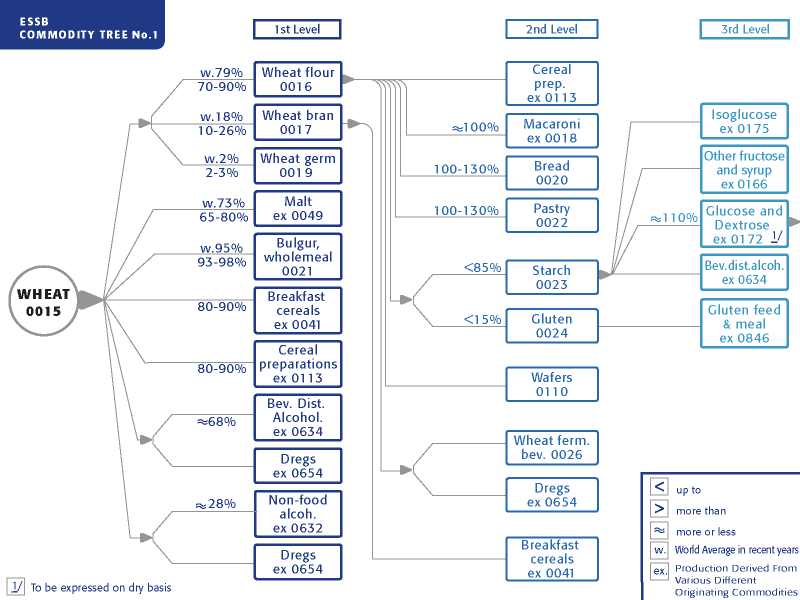
\includegraphics[scale = 0.3]{wheat_commodity_tree.png}
  \end{figure}

}



\end{document}
